\documentclass[11pt]{article}
\usepackage[a4paper,margin=1in]{geometry}
\usepackage{fontspec}
\setmainfont{Latin Modern Roman}
\setsansfont{Latin Modern Sans}
\setmonofont{DejaVu Sans Mono}[Scale=0.82]
\usepackage{newunicodechar}
\newunicodechar{→}{\ensuremath{\rightarrow}}
\newunicodechar{−}{\ensuremath{-}}
\newunicodechar{≈}{\ensuremath{\approx}}
\newunicodechar{∞}{\ensuremath{\infty}}
\newunicodechar{β}{\ensuremath{\beta}}
\newunicodechar{γ}{\ensuremath{\gamma}}
\newunicodechar{ε}{\ensuremath{\varepsilon}}
\newunicodechar{√}{\ensuremath{\surd}}
\newunicodechar{±}{\ensuremath{\pm}}
\newunicodechar{₁}{\ensuremath{_1}}
\newunicodechar{₂}{\ensuremath{_2}}
\newunicodechar{¹}{\textsuperscript{1}}
\newunicodechar{⁸}{\textsuperscript{8}}
\newunicodechar{⁹}{\textsuperscript{9}}
\newunicodechar{×}{\ensuremath{\times}}
\newunicodechar{·}{\ensuremath{\cdot}}
\usepackage{amsmath,amssymb}
\usepackage{microtype}
\usepackage{booktabs,tabularx,array}
\usepackage{graphicx}
\usepackage{enumitem}
\usepackage{needspace}
\usepackage{ragged2e}
\setlist{itemsep=2pt,topsep=4pt}
\usepackage{fvextra}
\usepackage[numbers,sort&compress]{natbib}
\usepackage{xcolor}
\definecolor{linkblue}{HTML}{1F5FA8}
\usepackage[colorlinks=true,linkcolor=linkblue,citecolor=linkblue,urlcolor=linkblue]{hyperref}
\usepackage{xurl}
\usepackage[font=small,labelfont=bf]{caption}
\usepackage{titlesec}
\usepackage{tocloft}
\renewcommand{\cftsecleader}{\cftdotfill{\cftdotsep}}
\titleformat{\section}{\large\bfseries}{\thesection}{0.8em}{}
\titleformat{\subsection}{\normalsize\bfseries}{\thesubsection}{0.8em}{}
\setlength{\parskip}{0.45em}
\setlength{\parindent}{0pt}
\renewcommand{\arraystretch}{1.18}

\title{\textbf{Decoder-Only Transformer from Scratch}\\[0.3em]\large Technical Report}
\author{Yash Singh}
\date{November 2026}

\begin{document}

\begin{titlepage}
\centering
\vspace*{2.2cm}
{\LARGE\bfseries Decoder-Only Transformer from Scratch\par}
\vspace{0.4cm}
{\large Technical Report\par}
\vspace{1.2cm}
{\large Yash Singh\par}
\vspace{0.3cm}
{November 2026\par}
\vspace{1.4cm}
\begin{minipage}{0.84\linewidth}
\itshape In my earlier projects, like LinkLens-V2 and FACTIFY, I used transformer models through libraries, and I always wanted to understand how they actually work underneath. So instead of using the libraries as they are, I built every part from scratch, from the tokenizer to the evaluation, and trained it at two sizes. This report documents the final models and their results; the blog series describes how I got there, including the mistakes along the way.
\end{minipage}
\vspace{1.2cm}

{\bfseries Abstract\par}
\vspace{0.3cm}
\begin{minipage}{0.84\linewidth}
\small\justifying\noindent
This report describes two decoder-only transformer language models, with 110M and 336M parameters, built from scratch, including a byte-level BPE tokenizer, rotary position embeddings, multi-head causal attention with a KV cache, and a tested training and evaluation pipeline. Both were trained on FineWeb-Edu (2.5B and 7.0B tokens) on two NVIDIA A30 GPUs, in about 4.6 and 34.7 hours. On held-out FineWeb-Edu text they reach 1.000 and 0.897 bits per byte, better than the size-matched GPT-2 models (1.009 and 0.926), and they outperform them on science and knowledge benchmarks (ARC, SciQ, OpenBookQA), where the 336M also beats GPT-2 large. On other kinds of text, on commonsense benchmarks and on LAMBADA they fall behind, and their 8-task zero-shot average is about one point below GPT-2 at both sizes. The results follow the training data: an educationally filtered corpus buys knowledge and in-domain modelling at the cost of breadth.
\end{minipage}

\vfill
{\small
\textbf{Code:} \href{https://github.com/Kevhand/decoder-only-transformer-from-scratch}{github.com/Kevhand/decoder-only-transformer-from-scratch}\\[0.25em]
\textbf{Models:} \href{https://huggingface.co/Kevhand}{huggingface.co/Kevhand}
\quad\textperiodcentered\quad
\textbf{Blog:} \href{https://yashksingh.hashnode.dev/}{yashksingh.hashnode.dev}\par}
\vspace{0.6cm}
\end{titlepage}

\setcounter{page}{1}
\pagenumbering{roman}
{\hypersetup{linkcolor=black}\tableofcontents}
\clearpage
\pagenumbering{arabic}

\section{Summary}

This project builds a GPT-style language model from scratch, tokenizer included, and trains it at two sizes on two GPUs. Apart from PyTorch's tensor operations and its fused attention kernel, every part is our own code: a byte-level BPE tokenizer, token embeddings, rotary position embeddings, multi-head causal attention with a KV cache, LayerNorm, the feed-forward network, and the training and evaluation pipeline, each with its own tests.

\begin{center}
\small
\begin{tabularx}{\linewidth}{>{\raggedright\arraybackslash}X>{\raggedright\arraybackslash}X>{\raggedright\arraybackslash}X}
\toprule
 & \textbf{110M} & \textbf{336M} \\
\midrule
Parameters & 110.3M & 335.9M \\
Layers × d\_\allowbreak{}model & 12 × 768 & 24 × 1,024 \\
Training data & 2.5B tokens of FineWeb-Edu & 7.0B tokens of FineWeb-Edu \\
Training time on 2× A30 & ≈ 4.6 h at 35\% MFU & ≈ 34.7 h at 39\% MFU \\
Held-out FineWeb-Edu, bits/\allowbreak{}byte & \textbf{1.000} (GPT-2 small: 1.009) & \textbf{0.897} (GPT-2 medium: 0.926; large: 0.880) \\
8-task zero-shot average & 40.6 (GPT-2 small: 41.5) & 44.9 (GPT-2 medium: 46.0) \\
\bottomrule
\end{tabularx}
\end{center}

\needspace{5\baselineskip}\textbf{Main results.}

\begin{itemize}
\item On text like their training data, both models beat the size-matched GPT-2, and the 336M comes within 0.017 bits/\allowbreak{}byte of GPT-2 large, a model 2.3× its size.
\item On science and school-knowledge benchmarks (ARC-Easy, ARC-Challenge, SciQ, OpenBookQA), both models beat the size-matched GPT-2, and the 336M beats GPT-2 large on all four.
\item They are weaker on narrative and general text: 0.06–0.11 bits/\allowbreak{}byte behind on Wikipedia and C4, behind on HellaSwag, PIQA and WinoGrande, and 9–11 points behind on LAMBADA. The overall benchmark average ends about 1 point below GPT-2 at both sizes.
\item Given a short, explicit passage, both use it like GPT-2 does (100\% with a supporting passage); they extract less from longer reading-comprehension passages and answer in full sentences rather than short spans.
\end{itemize}

The pattern follows the data: FineWeb-Edu is filtered for educational content, which buys knowledge and in-domain modelling at the cost of breadth. The rest of this report covers the tokenizer, the architecture, the data and training setup, every evaluation, and the engineering problems found along the way.

\section{Tokenizer}

Both models use a byte-level BPE tokenizer written from scratch~\citep{sennrich2016bpe,radford2019gpt2}: a 32,768-token vocabulary trained on FineWeb-Edu. It compresses held-out FineWeb-Edu to \textbf{about 4.6 bytes per token, on par with GPT-2's 50,257-token tokenizer} despite a vocabulary 35\% smaller, and encodes any UTF-8 text without unknown tokens.

\subsection{Design}

\begin{center}
\small
\begin{tabularx}{\linewidth}{l>{\raggedright\arraybackslash}X}
\toprule
\textbf{Component} & \textbf{Choice} \\
\midrule
Base vocabulary & The 256 byte values, at IDs 0–255 (token ID = byte value) \\
Special tokens & \texttt{[PAD]} 256, \texttt{[BOS]} 257, \texttt{[EOS]} 258, \texttt{[UNK]} 259. \texttt{[UNK]} is never produced, since every byte is in the base vocabulary \\
Vocabulary size & 32,768 (256 bytes + 4 special tokens + 32,508 merges) \\
Pre-tokenizer & Hand-written and Unicode-aware: splits letters, numbers and other symbols by Unicode category; attaches a leading space to the following word, number or symbol run; keeps newlines as their own chunk; splits the contractions 's, 're, 've, 'll, 'd, n't and 'm from the word they end \\
Merges & Learned within pre-token chunks only, never across them; applied at encode time lowest rank first \\
Stored state & Only the ordered merges, as pairs of token IDs; the vocabulary is rebuilt from them on load \\
Training data & A sample of FineWeb-Edu (sample-10BT) \\
\bottomrule
\end{tabularx}
\end{center}

The pre-tokenizer follows the same idea as GPT-2's regex~\citep{radford2019gpt2} but differs in one visible way: it splits off ``n't'' rather than ``'t'', so don't → ``Do'' + ``n't'' and aren't → `` are'' + ``n't'', keeping the base word whole.

\subsection{Training}

\begin{itemize}
\item Each document is pre-tokenized separately, in parallel worker processes, so chunks never span documents.
\item Training runs on the \textbf{distinct} chunks, each weighted by its frequency. This produces the same merges as training on every occurrence, about 6.6× faster.
\item Pair counts are updated incrementally: an index from each pair to the chunks containing it means a merge only recounts the affected chunks. The most frequent pair is taken from a max-heap with lazy deletion (stale entries are skipped when popped).
\item Chunks are processed in sorted order, so training is deterministic.
\end{itemize}

\subsection{Encoding and integration}

\begin{itemize}
\item \texttt{encode} returns raw token IDs. A chunk-to-IDs cache avoids re-running BPE on repeated chunks, making encoding about 2.4× faster.
\item The training data is packed as \texttt{[BOS] document [EOS]}, back to back, into 1,024-token sequences, so no padding is used. The model masks the \texttt{[PAD]} logit, so it can never be predicted.
\item The saved tokenizer records its format version, pre-tokenizer version and contraction list, and loading refuses a mismatch, so the same text can never be split differently from the training data.
\item Verified by exact encode–decode round trips, and by re-encoding 300 validation documents and checking they match the token shards exactly.
\end{itemize}

\subsection{Comparison with other tokenizers}

The same texts were encoded with each tokenizer. Compression is in bytes of UTF-8 text per token (higher means fewer tokens for the same text); every tokenizer round-tripped all four sets exactly.

\begin{center}
\footnotesize
\setlength{\tabcolsep}{3pt}
\begin{tabularx}{\linewidth}{>{\raggedright\arraybackslash}X>{\centering\arraybackslash}X>{\centering\arraybackslash}X>{\centering\arraybackslash}X>{\centering\arraybackslash}X>{\centering\arraybackslash}X>{\centering\arraybackslash}X>{\centering\arraybackslash}X}
\toprule
\textbf{Tokenizer} & \textbf{Vocabulary} & \textbf{FineWeb-Edu} & \textbf{Python code} & \textbf{Hindi} & \textbf{Numbers} & \textbf{Vocabulary used on FineWeb-Edu} & \textbf{Encoding speed (MB/\allowbreak{}s, 1 process)} \\
\midrule
Ours & 32,768 & 4.58 & 2.07 & 2.14 & 2.68 & 90.7\% & 0.89 \\
GPT-2 & 50,257 & 4.61 & 2.25 & 1.68 & 2.86 & 74.1\% & 14.13 \\
LLaMA-2~\citep{touvron2023llama2} & 32,000 & 3.99 & 3.60 & 2.42 & 1.63 & 57.5\% & 2.55 \\
GPT-4 (cl100k) & 100,277 & 4.69 & 4.58 & 2.62 & 2.40 & 40.9\% & 5.53 \\
\bottomrule
\end{tabularx}
\end{center}

Test sets: FineWeb-Edu documents from far past the tokenizer's training sample, Python standard-library source, Hindi Wikipedia articles, and generated number-heavy text (prices, dates, decimals). GPT-2 and GPT-4 were run through tiktoken and LLaMA-2 through Hugging Face transformers.

\begin{itemize}
\item \textbf{On its training domain, the tokenizer matches GPT-2 with a smaller vocabulary} (4.58 vs 4.61 bytes per token), and it uses 90.7\% of its vocabulary on FineWeb-Edu, against 74.1\% for GPT-2, so few entries are wasted.
\item \textbf{It beats GPT-2 on Hindi} (2.14 vs 1.68), but is behind LLaMA-2 and GPT-4, whose training data is far more multilingual.
\item \textbf{It is weakest on code}: runs of spaces are split into one token per space (see Limitations), which matters most for indentation.
\item \textbf{Encoding speed} reflects the implementation, not the algorithm: ours is pure Python, while tiktoken is written in Rust.
\end{itemize}

On a typical English sentence the splits are close to GPT-2's, differing mainly in contractions:

\begin{Verbatim}[fontsize=\footnotesize,frame=leftline,framesep=8pt,breaklines,breakanywhere=false,breaksymbolleft={}]
"Jane Austen’s novels weren't only about romance; they're about independence."
Ours   18 tokens  'J' 'ane' ' Aust' 'en' '’' 's' ' novels' ' were' "n't" ' only' ' about' ' romance' ';' ' they' "'re" ' about' ' independence' '.'
GPT-2  18 tokens  'Jane' ' Aust' 'en' <e2 80> <99> 's' ' novels' ' weren' "'t" ' only' ' about' ' romance' ';' ' they' "'re" ' about' ' independence' '.'
\end{Verbatim}

\subsection{Compression on the evaluation text}

The bits-per-byte evaluations also recorded how many tokens each tokenizer needed for exactly the same text, which gives a second comparison with GPT-2 on the four kinds of text the models were scored on.

\begin{figure}[ht]
\centering
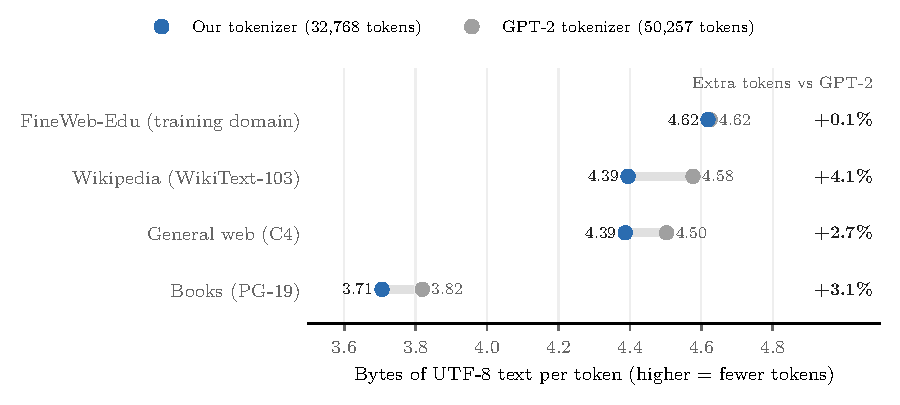
\includegraphics[width=\linewidth]{figures/tokenizer_compression.pdf}
\caption{Bytes of UTF-8 text per token on the evaluation text: our tokenizer matches GPT-2 on FineWeb-Edu but needs 2.7--4.1\% more tokens on other text. Source: domain\_results.json (token counts from the bits-per-byte evaluation; all GPT-2 sizes share one tokenizer, as do both of our models).}
\label{fig:compression}
\end{figure}

The tokenizer shows the same domain pattern as the models: it is as efficient as GPT-2's on the educational web text it was trained on, and less efficient on everything else. Bits per byte is unaffected by token counts, but more tokens means more computation per document and less text per 1,024-token context.

\subsection{Why results are reported in bits per byte}

Loss and perplexity are measured per token, and a token covers a different amount of text in each tokenizer, so they cannot be compared between models with different tokenizers. Bits per byte divides the total loss by the number of UTF-8 bytes in the text, which is identical for every model:

\begin{equation*}
\text{bits per byte} = \frac{\text{total loss (nats)}}{\ln 2 \times \text{bytes of text}} = \frac{\text{loss per token}}{\ln 2 \times \text{bytes per token}}
\end{equation*}

The difference matters in these results. On the books text, our 110M model has a lower loss per token than GPT-2 small (3.659 vs 3.732 nats, perplexity 38.8 vs 41.8), which would suggest it predicts books better. But our tokenizer splits that text into 3.1\% more tokens, each slightly easier to predict. Per byte, our model is worse: 1.424 vs 1.410 bits per byte. Comparing per-token numbers would have reversed the conclusion.

\subsection{What the vocabulary costs the model}

Every vocabulary entry needs a row in the token embedding matrix, which is shared with the output layer (weight tying), so it is counted once.

\begin{center}
\small
\begin{tabular}{lccc}
\toprule
\textbf{Model} & \textbf{Token embedding matrix} & \textbf{Parameters} & \textbf{Share of the model} \\
\midrule
Ours (110M) & 32,768 × 768 & 25.2M & 22.8\% \\
GPT-2 small (124M) & 50,257 × 768 & 38.6M & 31.0\% \\
Ours (336M) & 32,768 × 1,024 & 33.6M & 10.0\% \\
GPT-2 medium (355M) & 50,257 × 1,024 & 51.5M & 14.5\% \\
\bottomrule
\end{tabular}
\end{center}

At the same compression on FineWeb-Edu, the smaller vocabulary uses 13.4M fewer embedding parameters than GPT-2 small. The share shrinks as models grow, since the embedding grows with the model width while the transformer layers grow with width squared.

\subsection{Limitations}

\begin{itemize}
\item \textbf{Whitespace runs:} a space not followed by a letter, number or symbol becomes its own chunk, so indentation costs one token per space. This is the main reason code compresses worse than with GPT-2 (2.07 vs 2.25 bytes per token).
\item \textbf{Non-English scripts:} the vocabulary is fitted to English educational text. Hindi averages 2.14 bytes per token, under one Devanagari character (3 bytes) per token, so much of it falls back to raw bytes.
\item \textbf{Numbers:} the pre-tokenizer keeps digit runs together, but BPE then merges digits by frequency, so a number's split depends on its digits (2026 becomes `` 20'' + ``26'').
\item \textbf{Speed:} pure-Python encoding at under 1 MB/\allowbreak{}s per process; tokenizing the 7B-token training set relied on many parallel worker processes.
\end{itemize}

\section{Model architecture}

Both models are built from the same code: a decoder-only transformer~\citep{vaswani2017attention,radford2019gpt2} with pre-LayerNorm blocks~\citep{ba2016layernorm,xiong2020preln}, rotary position embeddings on queries and keys~\citep{su2021roformer}, a GELU feed-forward network~\citep{hendrycks2016gelu}, and an output layer tied to the token embedding~\citep{press2017tying}. Only the configuration differs. Every component is implemented from scratch in PyTorch (no nn.Transformer, nn.LayerNorm or nn.MultiheadAttention); the only fused library call is torch.nn.functional.scaled\_\allowbreak{}dot\_\allowbreak{}product\_\allowbreak{}attention.

\subsection{Configuration}

\begin{center}
\small
\begin{tabular}{lll}
\toprule
 & \textbf{110M} & \textbf{336M} \\
\midrule
Vocabulary & 32,768 & 32,768 \\
d\_\allowbreak{}model & 768 & 1,024 \\
Decoder blocks & 12 & 24 \\
Attention heads × head\_\allowbreak{}dim & 12 × 64 & 16 × 64 \\
FFN hidden size d\_\allowbreak{}ff & 3,072 (4×) & 4,096 (4×) \\
Context length & 1,024 & 1,024 \\
Total parameters & 110,254,592 & 335,898,624 \\
Non-embedding parameters & 85,088,768 & 302,344,192 \\
Embedding share of parameters & 22.8\% & 10.0\% \\
\bottomrule
\end{tabular}
\end{center}

\subsection{Forward pass}

\begin{Verbatim}[fontsize=\footnotesize,frame=leftline,framesep=8pt,breaklines,breakanywhere=false,breaksymbolleft={}]
token IDs (B, T)
  → token embedding                                   (B, T, d_model)
  → N × decoder block:
        h = x + W_O · Attention(RoPE(Q), RoPE(K), V),  with Q, K, V = projections of LN₁(x)
        y = h + FFN(LN₂(h))
  → final LayerNorm
  → LM head (weight tied to the embedding, own bias)   (B, T, vocab)
  → PAD logit set to −∞
\end{Verbatim}

\subsection{Components}

\begin{center}
\small
\begin{tabularx}{\linewidth}{l>{\raggedright\arraybackslash}X}
\toprule
\textbf{Component} & \textbf{Implementation} \\
\midrule
Token embedding & nn.Embedding with padding\_\allowbreak{}idx = PAD (ID 256); PAD row initialized to zero \\
Q, K, V projections & Three separate d\_\allowbreak{}model → d\_\allowbreak{}model linear layers with bias, reshaped to (B, heads, T, head\_\allowbreak{}dim) \\
Positional information & RoPE on Q and K only, base 10,000, interleaved (even, odd) pairs, 32 pairs per head; cos/\allowbreak{}sin tables precomputed for 1,024 positions in float32, registered as non-persistent buffers (not saved in checkpoints) \\
Attention & Multi-head causal attention via scaled\_\allowbreak{}dot\_\allowbreak{}product\_\allowbreak{}attention, scale 1/\allowbreak{}√64; a manual path (explicit scores, −∞ mask, softmax) with identical results is kept for inspecting attention weights \\
Output projection & W\_\allowbreak{}O, d\_\allowbreak{}model → d\_\allowbreak{}model with bias \\
Feed-forward & Linear (d\_\allowbreak{}model → 4·d\_\allowbreak{}model) → exact GELU → Linear (4·d\_\allowbreak{}model → d\_\allowbreak{}model), both with bias \\
Normalization & Custom LayerNorm (population variance, ε = 1e-5, learnable γ and β): pre-LN before attention and before the FFN in every block, plus one final LayerNorm after the last block \\
Output layer & nn.Linear sharing its weight matrix with the token embedding (saves 25.2M /\allowbreak{} 33.6M parameters), with its own bias; the PAD logit is masked to −∞ so PAD is never predicted and its row receives no gradient through the head \\
\bottomrule
\end{tabularx}
\end{center}

\textbf{KV cache.} Each block caches its keys after RoPE and its values, so a generation step only projects, rotates and attends for the new tokens. RoPE is applied to the new Q and K at their absolute offset (past\_\allowbreak{}len), and attention builds its causal mask from absolute positions, so a rectangular (new tokens × all keys) mask is supported. Attention has three paths: is\_\allowbreak{}causal=True for a fresh pass, no mask for a single new token (it may attend to every cached key), and an explicit position mask for a multi-token chunk on top of a cache. Mismatched cache lengths and cache lists of the wrong length raise errors.

\textbf{Mixed precision.} Training and bf16 evaluation run under torch.autocast with bfloat16. RoPE's tables are float32 and are not cast down, so the rotation itself runs in float32 and returns float32 Q and K; attention then runs in bf16 under autocast. Measured on head\_\allowbreak{}dim 64 across all 1,024 positions, this keeps the drift of a fixed-gap Q·K score at 0.12, against 0.19 when the tables are cast to bf16 first (0.0002 in pure float32).

\subsection{Initialization}

GPT-2 style:

\begin{center}
\small
\begin{tabularx}{\linewidth}{>{\raggedright\arraybackslash}X>{\raggedright\arraybackslash}X}
\toprule
\textbf{Parameter} & \textbf{Initialization} \\
\midrule
Token embedding (and so the tied LM head weight) & Normal(0, 0.02), PAD row zero \\
Linear weights & Normal(0, 0.02) \\
Residual projections (W\_\allowbreak{}O and the FFN's second layer) & Normal(0, 0.02 /\allowbreak{} √(2N)): 0.0041 for the 110M (N = 12), 0.0029 for the 336M (N = 24) \\
Linear biases & Zero \\
LayerNorm γ /\allowbreak{} β & One /\allowbreak{} zero \\
\bottomrule
\end{tabularx}
\end{center}

The embedding is initialized last, after the linear layers, because the tied LM head is an nn.Linear and would otherwise overwrite the shared matrix and its zero PAD row. With this initialization the initial logits have a standard deviation of about 0.16 and the initial loss matches the uniform baseline ln(V − 1); with PyTorch's default N(0, 1) embedding the logits' standard deviation was about 8 and the initial loss on a 1,000-token test model was 56.4 instead of 6.9.

\subsection{Parameters}

\begin{center}
\small
\begin{tabular}{lll}
\toprule
\textbf{Part} & \textbf{110M} & \textbf{336M} \\
\midrule
Token embedding /\allowbreak{} tied LM head weight & 25.17M (22.8\%) & 33.55M (10.0\%) \\
Attention (Q, K, V, W\_\allowbreak{}O), all blocks & 28.35M (25.7\%) & 100.76M (30.0\%) \\
Feed-forward, all blocks & 56.67M (51.4\%) & 201.45M (60.0\%) \\
LayerNorms (2 per block + final) & 0.04M & 0.10M \\
LM head bias & 0.03M & 0.03M \\
Per decoder block & 7.09M & 12.60M \\
\bottomrule
\end{tabular}
\end{center}

\subsection{Verification}

Each component has its own test file, and the whole suite passes on CPU in about 93 seconds. The tests check behaviour, not just shapes, and each property test has a negative control so it can fail:

\begin{itemize}
\item \textbf{Against references:} LayerNorm matches nn.LayerNorm in the forward pass and in all gradients (with initial and with random γ/\allowbreak{}β); the FFN matches a hand computation; the fused attention path matches the manual path in outputs (difference 2.4e-7) and gradients.
\item \textbf{RoPE:} each pair is rotated by position × frequency (hand computation); vector length is preserved; position 0 is the identity; Q·K depends only on the relative position (same gap: difference 6e-8, different gap: 0.149); out-of-range, negative-offset and odd-head\_\allowbreak{}dim inputs are rejected.
\item \textbf{Causality:} changing token 8 leaves the outputs and logits at positions 0–7 unchanged and changes every position from 8 on, in both attention paths.
\item \textbf{KV cache:} token-by-token and uneven chunked processing (3 + 4 + 5 tokens) match a full pass at block and model level, in both attention paths.
\item \textbf{Model:} Pre-LN wiring (with sublayer outputs zeroed, a block is exactly the identity); weight tying survives a save/\allowbreak{}load round trip; the PAD row stays exactly zero through AdamW steps with weight decay; initial loss within 0.1 of ln(V − 1); a one-batch overfit goes from 6.89 to 0.0096 in 150 steps.
\end{itemize}

On the trained checkpoints, cached and uncached generation pick the same tokens over 64 steps, with a maximum logit difference of 2.2e-5 (110M) and 2.3e-5 (336M) in float32.

\section{Data}

Both models are trained on \textbf{FineWeb-Edu}~\citep{penedo2024fineweb} (HuggingFaceFW/\allowbreak{}fineweb-edu, the sample-10BT subset): English web pages filtered by a classifier for educational value, streamed from the Hugging Face Hub.

\begin{center}
\small
\begin{tabular}{lll}
\toprule
 & \textbf{110M} & \textbf{336M} \\
\midrule
Training tokens & 2,499,805,184 (2.50B) & 6,999,769,088 (7.00B) \\
Passes over the data & 1 & 1 \\
Tokens per parameter & 22.7 & 20.8 \\
\bottomrule
\end{tabular}
\end{center}

Both models get roughly 20 tokens per parameter, about the compute-optimal ratio from the Chinchilla scaling work~\citep{hoffmann2022chinchilla}, and every training token is seen once.

\textbf{Tokenization and packing.} The documents are tokenized with the project's byte-level BPE tokenizer (see Tokenizer), in parallel worker processes. Each document becomes [BOS] + tokens + [EOS], and documents are packed back to back with no padding, so a 1,024-token training window can span several documents and no compute is spent on PAD. Tokens are stored as uint16 (the 32,768-token vocabulary fits) in .npy shards of 100M tokens (200 MB each), with a manifest recording the shards, the token counts, the tokenizer and how many source documents were consumed.

\textbf{Two datasets, one stream.} The 2.5B-token dataset was tokenized first, for the 110M. For the 336M it was extended to 7B tokens by resuming from the manifest: tokenization continued from the first document not yet used, appending new training shards. So the 336M's data is a superset of the 110M's, both start from the same documents, and the validation shard is identical for both runs.

\textbf{Validation split.} The first 10,121,940 tokens of the stream (about 10.1M) form the validation shard, and everything after goes to training shards, so no validation document is ever trained on. During training, validation loss and bits per byte are computed every 250 steps on a fixed slice from the start of this shard: 64 micro-batches, which is 1.05M tokens for the 110M (micro-batch 16) and 0.52M tokens for the 336M (micro-batch 8).

\textbf{Held-out evaluation text.} The final evaluations use separate text: FineWeb-Edu documents from \textbf{after document 7,500,000} of the same stream, beyond everything used for training (and for the tokenizer). 1,036 documents (5.0 MB) are scored, each starting with the model's start token and split into non-overlapping 1,024-token windows. This differs from the in-training validation (packed windows that cross document boundaries), so the two sets of numbers are close but not identical: 1.0240 vs 1.0004 bits per byte for the 110M, and 0.9120 vs 0.8966 for the 336M.

\textbf{Data loading.} The shards are memory-mapped and read as one long stream in a shuffled shard order (seeded per epoch). Micro-step k on GPU r reads chunk k × world\_\allowbreak{}size + r, a pure function of the step, so the two GPUs never read the same tokens and a resumed run continues exactly where it stopped. Each chunk is micro\_\allowbreak{}batch × 1,024 + 1 tokens, giving inputs and next-token targets offset by one.

\section{Training}

Both models were trained with the same script (train.py) on one server with \textbf{2× NVIDIA A30 (24 GB)}, using PyTorch DistributedDataParallel launched by torchrun, bfloat16 autocast, and torch.compile.

\subsection{Setup}

\begin{center}
\small
\begin{tabularx}{\linewidth}{l>{\raggedright\arraybackslash}X>{\raggedright\arraybackslash}X}
\toprule
 & \textbf{110M} & \textbf{336M} \\
\midrule
Tokens per optimizer step & 524,288 (2¹⁹) & 524,288 (2¹⁹) \\
Per step & 16 seq × 1,024 × 2 GPUs × 16 accumulation & 8 seq × 1,024 × 2 GPUs × 32 accumulation \\
Optimizer steps & 4,768 & 13,351 \\
Peak learning rate & 6e-4 & 3e-4 \\
Warmup & 143 steps (3\%) & 400 steps (3\%) \\
Final learning rate & 6e-5 (10\% of peak) & 3e-5 (10\% of peak) \\
Mean throughput & 150,796 tokens/\allowbreak{}s & 56,071 tokens/\allowbreak{}s \\
Time per step & 3.47 s & 9.34 s \\
MFU & 35.4\% & 39.4\% \\
Training time (steps only) & ≈ 4.6 h & ≈ 34.7 h \\
Training compute & ≈ 1.9 × 10¹⁸ FLOPs & ≈ 1.6 × 10¹⁹ FLOPs \\
\bottomrule
\end{tabularx}
\end{center}

Shared settings:

\begin{itemize}
\item \textbf{Optimizer:} AdamW with~\citep{loshchilov2019adamw} β = (0.9, 0.95), ε = 1e-8 (fused CUDA implementation). Weight decay 0.1 on every matrix (all linear weights and the tied embedding); none on biases or LayerNorm parameters.
\item \textbf{Schedule:} linear warmup over the first 3\% of steps, then cosine decay to 10\% of the peak learning rate at the last step.
\item \textbf{Gradient clipping} at a global norm of 1.0.
\item \textbf{Loss:} cross-entropy over all positions of the packed windows.
\item \textbf{Precision:} bf16 autocast for the forward and backward pass; float32 master weights and optimizer state.
\item \textbf{Checkpoints} every 250 steps for the 110M and every 100 steps for the 336M (the longer run), with resumable data order; weights-only copies kept every 1,000 steps.
\item \textbf{Monitoring:} training loss, learning rate, gradient norm and throughput every 10 steps; validation loss and bits per byte every 250 steps; a sampled completion of ``The most important thing about learning is'' every 500 steps.
\end{itemize}

The 336M uses half the peak learning rate of the 110M, a common adjustment for a larger model, and a micro-batch of 8 so that its activations fit in 24 GB, with twice the gradient accumulation to keep the same 2¹⁹-token batch. It was launched with PYTORCH\_\allowbreak{}CUDA\_\allowbreak{}ALLOC\_\allowbreak{}CONF=\allowbreak{}expandable\_\allowbreak{}segments:True to reduce memory fragmentation.

\textbf{MFU} (model FLOPs utilization~\citep{chowdhery2022palm}) is measured against the A30's 165 TFLOPS bf16 peak per GPU, counting 6N FLOPs per token for the weights plus 12 · layers · d\_\allowbreak{}model · context for attention. Before the 110M run, a 30-step benchmark showed what torch.compile is worth:

\begin{center}
\small
\begin{tabular}{lccc}
\toprule
\textbf{110M, 30-step benchmark} & \textbf{Throughput} & \textbf{MFU} & \textbf{Peak memory per GPU} \\
\midrule
Eager & 91,544 tokens/\allowbreak{}s & 21.5\% & 18.9 GB \\
torch.compile & 153,375 tokens/\allowbreak{}s & 36.0\% & 15.5 GB \\
\bottomrule
\end{tabular}
\end{center}

Compiling made training 1.68× faster and used less memory, so both runs used it; uncompiled, the 110M run would have taken about 7.6 hours instead of 4.6.

\subsection{The runs}

Both runs went from start to finish without a restart, a loss spike or a divergence. The initial loss was 10.55 (110M) and 10.65 (336M), close to ln(32,767) = 10.40 for a uniform guess over every token except PAD. After warmup the gradient norm settled quickly: its median over the run was 0.27 for the 110M and 0.23 for the 336M, and it went above the clipping threshold of 1.0 only a handful of times, all within a few hundred steps of the end of warmup (2 logged steps for the 110M, 4 for the 336M, at most 1.07).

\begin{center}
\small
\begin{tabular}{lll}
\toprule
\textbf{Validation (in-training set)} & \textbf{110M} & \textbf{336M} \\
\midrule
After 0.5B tokens (step 1,000) & 1.197 bits/\allowbreak{}byte & 1.222 bits/\allowbreak{}byte \\
After 1.0B tokens (step 2,000) & 1.102 & 1.084 \\
After 2.5B tokens (step 4,750) & 1.025 & 0.989 \\
Final & \textbf{1.024} (loss 3.262) & \textbf{0.912} (loss 2.882) \\
\bottomrule
\end{tabular}
\end{center}

The 336M starts slower, with a lower peak learning rate and a longer warmup, overtakes the 110M at about 0.75B tokens (step 1,500), and at 2.5B tokens, where the 110M's training ended, it is already 0.035 bits/\allowbreak{}byte better, even though its learning rate at that point is still about three-quarters of its peak (2.3e-4) while the 110M's has fully decayed. The remaining 4.5B tokens take it from 0.989 to 0.912. Both curves are still decreasing at the end: neither model has reached the limit of what more data would give it.

\begin{figure}[ht]
\centering
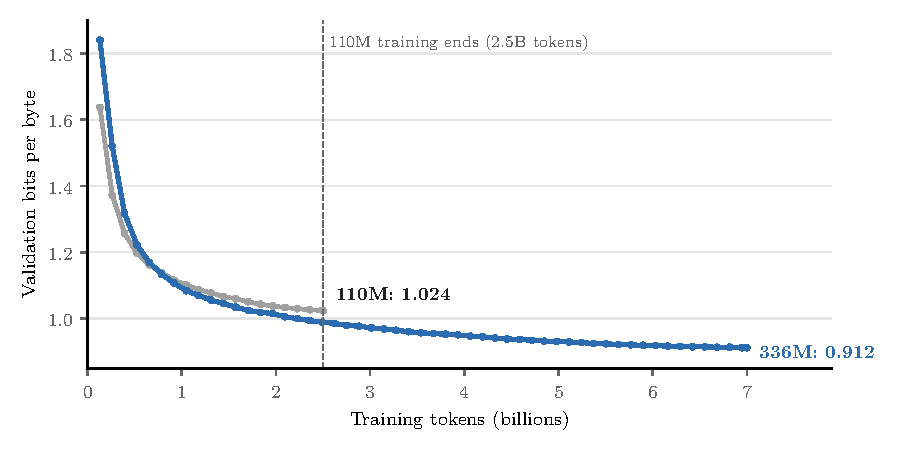
\includegraphics[width=\linewidth]{figures/validation_curves.pdf}
\caption{Validation bits per byte during training (in-training validation set, every 250 steps; lower is better). The 336M reaches 0.912; the 110M stops at 1.024 after 2.5B tokens. Source: log\_110m.jsonl and log\_336m.jsonl, 20 and 54 points.}
\label{fig:validation}
\end{figure}

The completion of the fixed prompt at the end of each run (temperature 0.8, top-k 50):

\begin{itemize}
\item \textbf{110M:} ``The most important thing about learning is that you can’t do anything without learning. Learning is all about memorizing and remembering…''
\item \textbf{336M:} ``The most important thing about learning is that it is not easy. You have to change every single aspect of your life. You have to learn t…''
\end{itemize}

\section{Evaluation}

Every evaluation runs our two models and the three GPT-2 models from Hugging Face~\citep{radford2019gpt2} (small 124M, medium 355M, large 774M) on identical data with identical scoring. GPT-2 small is the size match for the 110M and GPT-2 medium for the 336M. GPT-2 was trained by OpenAI on WebText, a broader web corpus than FineWeb-Edu, so these comparisons measure both the models and their training data.

\subsection{Language modelling: bits per byte}

On the held-out FineWeb-Edu text (1,036 documents, 5.0 MB, from after everything used for training):

\begin{center}
\small
\begin{tabular}{lcccc}
\toprule
\textbf{Model} & \textbf{Bits/\allowbreak{}byte} & \textbf{Loss/\allowbreak{}token} & \textbf{Perplexity} & \textbf{Bytes/\allowbreak{}token} \\
\midrule
Ours (110M) & \textbf{1.0004} & 3.2032 & 24.61 & 4.62 \\
GPT-2 small (124M) & 1.0093 & 3.2358 & 25.43 & 4.63 \\
Ours (336M) & \textbf{0.8966} & 2.8708 & 17.65 & 4.62 \\
GPT-2 medium (355M) & 0.9262 & 2.9694 & 19.48 & 4.63 \\
GPT-2 large (774M) & 0.8801 & 2.8215 & 16.80 & 4.63 \\
\bottomrule
\end{tabular}
\end{center}

Bits per byte is the comparable measure, since each model uses its own tokenizer (see Tokenizer for why loss per token can mislead). On text like its training data, the 110M is slightly better than GPT-2 small, and the 336M is 0.030 bits/\allowbreak{}byte better than GPT-2 medium and within 0.017 of GPT-2 large, a model 2.3× its size.

\subsection{Bits per byte by kind of text}

The same measurement on three other kinds of text: Wikipedia~\citep{merity2017wikitext} (WikiText-103 test, 1.2 MB), books~\citep{rae2020pg19} (PG-19 test, 5.1 MB, a slice of each book starting 20\% in) and general web text~\citep{raffel2020c4} (C4 validation, 5.0 MB).

\begin{center}
\small
\begin{tabular}{lcccc}
\toprule
\textbf{Model} & \textbf{FineWeb-Edu} & \textbf{Wikipedia} & \textbf{Books} & \textbf{General web (C4)} \\
\midrule
Ours (110M) & \textbf{1.0004} & 1.1257 & 1.4244 & 1.1832 \\
GPT-2 small (124M) & 1.0093 & \textbf{1.0155} & \textbf{1.4098} & \textbf{1.0968} \\
Ours (336M) & \textbf{0.8966} & 0.9980 & 1.2961 & 1.0741 \\
GPT-2 medium (355M) & 0.9262 & \textbf{0.9212} & \textbf{1.2489} & \textbf{1.0138} \\
GPT-2 large (774M) & 0.8801 & 0.8706 & 1.2159 & 0.9681 \\
\bottomrule
\end{tabular}
\end{center}

Outside the training domain the order reverses: GPT-2 is better on all three, by 0.11 (110M vs small) and 0.08 (336M vs medium) bits/\allowbreak{}byte on Wikipedia, 0.09 and 0.06 on C4, and 0.01 and 0.05 on books. FineWeb-Edu is filtered towards educational web pages, so text that looks different (encyclopedic formatting, fiction, everyday web pages) is less familiar to our models. Scale still helps everywhere: the 336M improves on the 110M by 0.10–0.13 bits/\allowbreak{}byte in every domain.

\subsection{Zero-shot benchmarks}

Eight standard tasks from EleutherAI's lm-evaluation-harness~\citep{eval-harness}, run through a wrapper around our model class, in float32, zero-shot. Before trusting the wrapper, it was run on GPT-2 small next to the harness's own Hugging Face model: all 14 task/\allowbreak{}metric pairs agreed within 0.1 points.

\begin{center}
\footnotesize
\setlength{\tabcolsep}{3pt}
\resizebox{\linewidth}{!}{\begin{tabular}{lccccccccc}
\toprule
\begin{tabular}[t]{@{}c@{}}\textbf{Model}\end{tabular} & \begin{tabular}[t]{@{}c@{}}\textbf{HellaSwag}\\ \citep{zellers2019hellaswag}\end{tabular} & \begin{tabular}[t]{@{}c@{}}\textbf{PIQA}\\ \citep{bisk2020piqa}\end{tabular} & \begin{tabular}[t]{@{}c@{}}\textbf{ARC-e}\\ \citep{clark2018arc}\end{tabular} & \begin{tabular}[t]{@{}c@{}}\textbf{ARC-c}\\ \citep{clark2018arc}\end{tabular} & \begin{tabular}[t]{@{}c@{}}\textbf{WinoGrande}\\ \citep{sakaguchi2020winogrande}\end{tabular} & \begin{tabular}[t]{@{}c@{}}\textbf{SciQ}\\ \citep{welbl2017sciq}\end{tabular} & \begin{tabular}[t]{@{}c@{}}\textbf{OpenBookQA}\\ \citep{mihaylov2018openbookqa}\end{tabular} & \begin{tabular}[t]{@{}c@{}}\textbf{LAMBADA}\\ \citep{paperno2016lambada}\end{tabular} & \begin{tabular}[t]{@{}c@{}}\textbf{Average}\end{tabular} \\
\midrule
Ours (110M) & 29.5 & 60.1 & \textbf{43.1} & \textbf{24.1} & 51.7 & \textbf{65.4} & \textbf{28.0} & 22.8 & 40.6 \\
GPT-2 small (124M) & \textbf{31.1} & \textbf{62.6} & 39.5 & 22.7 & \textbf{51.8} & 64.4 & 27.2 & \textbf{32.6} & \textbf{41.5} \\
Ours (336M) & 35.4 & 63.3 & \textbf{48.3} & \textbf{28.0} & 51.6 & \textbf{70.4} & \textbf{31.8} & 30.7 & 44.9 \\
GPT-2 medium (355M) & \textbf{39.4} & \textbf{66.4} & 43.6 & 25.1 & \textbf{53.2} & 67.2 & 30.2 & \textbf{43.1} & \textbf{46.0} \\
GPT-2 large (774M) & 45.3 & 69.2 & 46.6 & 25.1 & 55.5 & 69.3 & 31.2 & 47.7 & 48.7 \\
\bottomrule
\end{tabular}}
\end{center}

Accuracy in \%, acc\_\allowbreak{}norm where the task has it, otherwise acc. Standard errors: about ±0.5 (HellaSwag), ±1.0–1.5 (PIQA, ARC, WinoGrande, SciQ), ±2.0 (OpenBookQA) and ±0.6–0.7 (LAMBADA). Chance is 25\% for the four-choice tasks, 50\% for PIQA and WinoGrande, 0\% for LAMBADA.

The results split cleanly by kind of task. On the \textbf{science and school-knowledge} tasks (ARC-Easy, ARC-Challenge, SciQ, OpenBookQA), both of our models beat their size-matched GPT-2, and the 336M beats GPT-2 large on all four (ARC-Easy 48.3 vs 46.6, ARC-Challenge 28.0 vs 25.1, SciQ 70.4 vs 69.3, OpenBookQA 31.8 vs 31.2). That's what FineWeb-Edu's filtering selects for. On \textbf{everyday commonsense and narrative} tasks (HellaSwag, PIQA, WinoGrande) GPT-2 is ahead, and on \textbf{LAMBADA}, which needs the last word of a story passage, it is far ahead (10 to 12 points). The averages end up about 1 point below GPT-2 at both sizes: 40.6 vs 41.5 and 44.9 vs 46.0.

HellaSwag was also measured with the project's own evaluate.py, which normalizes by tokens instead of bytes: 27.25\% (110M), 32.87\% (336M), 29.52\% (GPT-2 small, matching its published figure), 37.67\% (medium) and 43.12\% (large). The ordering is the same as in the harness.

\subsection{Generation}

The same prompts were completed by every model with greedy decoding, temperature sampling (0.8, top-k 50) and nucleus sampling (0.8, top-p 0.9); the full outputs are in results/\allowbreak{}eval\_\allowbreak{}report.md. Greedy decoding loops for every model at these sizes. Factual prompts show the domain difference: for ``The capital of France is'', the 336M's greedy completion is ``Paris.'', the only model to answer directly (GPT-2 medium continues ``a city of the future'', GPT-2 large ``a city of contrasts''), while the 110M produces a circular ``the capital of the French Republic''.

\subsection{Generation speed}

Batch 1, tokens per second while generating from a short prompt (A30, bf16; evaluate.py's speed task):

\begin{center}
\small
\begin{tabular}{lccc}
\toprule
\textbf{Model} & \textbf{With KV cache} & \textbf{Without cache} & \textbf{Speedup} \\
\midrule
Ours (110M) & 98.4 & 97.2 & 1.0× \\
GPT-2 small (124M) & 141.9 & 117.5 & 1.2× \\
Ours (336M) & 49.7 & 50.0 & 1.0× \\
GPT-2 medium (355M) & 77.1 & 62.5 & 1.2× \\
GPT-2 large (774M) & 53.6 & 37.5 & 1.4× \\
\bottomrule
\end{tabular}
\end{center}

At batch size 1 the time per token is dominated by launching many small GPU operations rather than by arithmetic. Hugging Face's GPT-2 launches fewer of them per layer (one fused Q/\allowbreak{}K/\allowbreak{}V projection, for example, where ours has three), so it is faster at the same size, and the KV cache saves comparatively more of its time. The KV cache correctness and the fix that made our cache faster than recomputing are under Engineering problems and fixes.

\section{Using context}

The benchmarks above mostly test what a model already knows. Three further tests (context\_\allowbreak{}eval.py) check whether the models \textbf{use} information given in the prompt. The same data and scoring are used for all five models.

\subsection{LAMBADA: the last word of a passage}

5,153 passages (OpenAI version)~\citep{paperno2016lambada} whose last word is easy to guess from the whole passage but hard from the last sentence alone. A passage counts as correct only if greedy decoding produces every token of the word.

\begin{center}
\small
\begin{tabular}{lll}
\toprule
\textbf{Model} & \textbf{Accuracy} & \textbf{Perplexity of the target word} \\
\midrule
Ours (110M) & 22.38\% & 158.9 \\
GPT-2 small (124M) & \textbf{30.93\%} & \textbf{38.9} \\
Ours (336M) & 30.55\% & 51.7 \\
GPT-2 medium (355M) & \textbf{41.41\%} & \textbf{17.8} \\
GPT-2 large (774M) & 47.31\% & 13.0 \\
\bottomrule
\end{tabular}
\end{center}

This is our models' weakest result: about 9 and 11 points behind the size-matched GPT-2, and the 336M only reaches GPT-2 small. LAMBADA passages are taken from novels, and keeping track of characters and events through a story is a skill FineWeb-Edu's educational pages rarely train; the books bits-per-byte result points the same way.

\subsection{SQuAD: reading comprehension}

1,000 SQuAD v1.1 questions~\citep{rajpurkar2016squad}, each with its Wikipedia paragraph and two worked examples (question → short answer) in front. The model generates an answer until the first newline or 20 tokens. Each question is also asked closed book, without the paragraph, so the gain from reading is visible.

\begin{center}
\small
\begin{tabularx}{\linewidth}{l>{\centering\arraybackslash}X>{\centering\arraybackslash}X>{\centering\arraybackslash}X>{\centering\arraybackslash}X}
\toprule
\textbf{Model} & \textbf{EM, with passage} & \textbf{F1, with passage} & \textbf{F1, without passage} & \textbf{F1 gain from passage} \\
\midrule
Ours (110M) & 0.1\% & 8.3\% & 4.6\% & +3.6 pts \\
GPT-2 small (124M) & 9.3\% & 19.8\% & 4.8\% & +15.0 pts \\
Ours (336M) & 3.2\% & 14.6\% & 6.3\% & +8.3 pts \\
GPT-2 medium (355M) & 24.0\% & 36.4\% & 8.0\% & +28.4 pts \\
GPT-2 large (774M) & 32.3\% & 45.7\% & 8.2\% & +37.5 pts \\
\bottomrule
\end{tabularx}
\end{center}

Exact match and F1 punish one thing our models do: they answer in full sentences. Their answers average 13.4 (110M) and 11.8 (336M) words against 4–5 for GPT-2, so a correct answer inside a sentence still scores near zero. A looser check, whether a correct answer appears anywhere in the output as whole words, separates \textbf{not finding} the answer from \textbf{phrasing} it badly:

\begin{center}
\small
\begin{tabularx}{\linewidth}{l>{\centering\arraybackslash}X>{\centering\arraybackslash}X>{\centering\arraybackslash}X>{\centering\arraybackslash}X}
\toprule
\textbf{Model} & \textbf{Answer found, with passage} & \textbf{Without passage} & \textbf{Gain from passage} & \textbf{Answer length (words)} \\
\midrule
Ours (110M) & 8.9\% & 0.8\% & +8.1 pts & 13.4 \\
GPT-2 small (124M) & 16.4\% & 1.2\% & +15.2 pts & 5.0 \\
Ours (336M) & \textbf{18.3\%} & 2.0\% & +16.3 pts & 11.8 \\
GPT-2 medium (355M) & 31.1\% & 3.2\% & +27.9 pts & 4.0 \\
GPT-2 large (774M) & 42.5\% & 3.0\% & +39.5 pts & 4.2 \\
\bottomrule
\end{tabularx}
\end{center}

With the looser check the 336M finds the answer more often than GPT-2 small (18.3\% vs 16.4\%), but it still finds it far less often than GPT-2 medium (31.1\%). Part of the EM gap is format, then, and most of it is real: our models also extract less from the passage. The two worked examples did not get either model to copy the short-answer format; its training text contains few question-and-answer pairs of that kind. A typical 336M answer: \emph{``Super Bowl 50 was held on February 7, 2016, at the San Francisco Bay Area. The game…''} (correct, and scored 0 by exact match).

\subsection{Knowing, reading, and following the context}

25 simple fact questions (``What is the capital of Japan?'': Tokyo or Osaka), each asked three ways. The model is scored by which of the two answers it finds more likely: with no passage (does it know?), after a passage stating the true answer (does it read?), and after a passage stating the false one (does it follow the context or its memory?).

\begin{center}
\small
\begin{tabularx}{\linewidth}{l>{\centering\arraybackslash}X>{\centering\arraybackslash}X>{\centering\arraybackslash}X}
\toprule
\textbf{Model} & \textbf{Knows it (no passage)} & \textbf{Reads it (true passage)} & \textbf{Follows a false passage} \\
\midrule
Ours (110M) & 80\% & 100\% & 92\% \\
GPT-2 small (124M) & 68\% & 96\% & 96\% \\
Ours (336M) & 80\% & 100\% & 96\% \\
GPT-2 medium (355M) & 80\% & 100\% & 100\% \\
GPT-2 large (774M) & 84\% & 100\% & 100\% \\
\bottomrule
\end{tabularx}
\end{center}

With 25 questions, one question is 4 points, so these are coarse. The 110M knows more of these facts than GPT-2 small (80\% vs 68\%) and as many as GPT-2 medium, consistent with its strength on the knowledge benchmarks. All models read a supporting passage almost perfectly. Given a passage that contradicts what they know, all of them mostly follow the passage; the 110M keeps its own answer on 2 of the 25 questions, the 336M and GPT-2 small on 1, GPT-2 medium and large on none.

Taken together: with a short, explicit passage our models use the context as well as GPT-2 does, but on longer and less structured context (stories, a Wikipedia paragraph answered in free form) they are clearly weaker. That's consistent with their training data: lots of explanatory text, few narratives, and little question-and-answer formatting.

\section{Engineering problems and fixes}

The problems that changed the code or the results, in the order they came up.

\begin{center}
\small
\begin{tabularx}{\linewidth}{>{\raggedright\arraybackslash}X>{\raggedright\arraybackslash}X>{\raggedright\arraybackslash}X>{\raggedright\arraybackslash}X}
\toprule
\textbf{Problem} & \textbf{How it showed} & \textbf{Fix} & \textbf{Effect} \\
\midrule
Initial loss far too high & Untrained 1,000-token test model started at a loss of 56.4 instead of ln(1000) = 6.9 & GPT-2-style initialization (std 0.02, scaled residual projections), embedding initialized last because of weight tying & Initial loss 6.90, logits' std 8.2 → 0.16 \\
PAD row of the tied matrix could change & padding\_\allowbreak{}idx protects the embedding lookup, but the tied LM head still gave the PAD row gradients & PAD logit set to −∞, PAD excluded from targets, row initialized to zero & Row stays exactly 0 through AdamW with weight decay (tested) \\
A test passed while printing NaN & Cache-equivalence max difference printed nan: −∞ − (−∞) on the PAD column, while allclose treats equal infinities as close & Compare non-PAD logits only & Real differences again (2.8e-7) \\
KV cache could not handle generation & First RoPE always started at position 0; the attention mask was a sliced square, wrong when Q is shorter than K & Absolute offsets in RoPE, keys cached after rotation, mask built from absolute positions & Token-by-token and chunked runs match a full pass to \textasciitilde{}1e-7 \\
Attention memory & Manual attention stores (B, heads, T, T) weights: 48 MB (110M) /\allowbreak{} 64 MB (336M) per layer per sequence in float32 & scaled\_\allowbreak{}dot\_\allowbreak{}product\_\allowbreak{}attention, with the manual path kept for inspection & Same results (2.4e-7), far less memory \\
Slow eager training & 110M benchmark at 91.5k tokens/\allowbreak{}s, MFU 21.5\% & torch.compile & 153k tokens/\allowbreak{}s, MFU 36.0\%, 1.68× faster, less memory \\
336M memory & 24 GB per A30 & Micro-batch 8 with 32 accumulation steps; expandable\_\allowbreak{}segments allocator & Same 2¹⁹-token batch, 39.4\% MFU \\
KV cache slower than no cache & Full-context generation: 89.4 vs 92.9 tokens/\allowbreak{}s (110M), 46.3 vs 47.9 (336M) & A single new token skips the mask (it may see every cached key), instead of building aranges and a mask in every layer at every step & 96.8 vs 93.1 (1.04×) and 49.8 vs 49.0 (1.02×); up to 1.08× in the last quarter of the context \\
bf16 vs float32 benchmark scores & Harness results in bf16 differed from float32 by up to 1.8 points (LAMBADA) & All reported harness numbers re-run in float32; our wrapper checked against the harness's own GPT-2 & Wrapper within 0.1 points on all 14 task/\allowbreak{}metric pairs \\
SQuAD exact match undercounted our models & Full-sentence answers containing the right answer scored 0 & Added an ``answer found'' check and answer length & 336M: 3.2\% EM, but 18.3\% answer found \\
\bottomrule
\end{tabularx}
\end{center}

The tokenizer had its own set of speed problems (weighted distinct-chunk training, about 6.6× faster; an encode cache, about 2.4×; a lazy-deletion heap and incremental pair counts), described under Tokenizer.

One decision that wasn't a bug: RoPE keeps its rotation in float32 under bf16 autocast instead of casting its tables down. Measured on head\_\allowbreak{}dim 64 across 1,024 positions, this lowers the drift of a fixed-gap Q·K score from 0.19 to 0.12.

The code fixes are covered by tests in the final suite (the KV-cache speed fix by the benchmark in results/\allowbreak{}kv\_\allowbreak{}cache\_\allowbreak{}report.md), and the suite was run before and after the attention change.

\section{Limitations and next steps}

\subsection{Limitations}

\begin{itemize}
\item \textbf{Narrow training data.} FineWeb-Edu makes both models strong on educational and science text and on knowledge benchmarks, but weaker than GPT-2 on fiction, Wikipedia-style text and general web text (0.06–0.11 bits/\allowbreak{}byte), on commonsense tasks, and especially on LAMBADA (9–11 points behind the size-matched GPT-2).
\item \textbf{Base models only.} Neither model is instruction-tuned. They don't follow a question-and-answer format from two examples (SQuAD answers average 12–13 words), and greedy decoding falls into repetition, as it does for GPT-2 at these sizes.
\item \textbf{Context length.} 1,024 tokens. The RoPE tables stop at position 1,023 and longer inputs are rejected; no context extension was tried.
\item \textbf{Tokenizer.} Each run of spaces costs a token per space, Hindi and other non-Latin scripts fall back to bytes, and numbers split irregularly (see Tokenizer).
\item \textbf{One run per size.} No repeated seeds and no ablations, so small differences (a point on a benchmark, a few questions in the 25-question test) are within noise.
\item \textbf{Inference speed.} At batch 1, our implementation is slower than Hugging Face's GPT-2 at the same size (98 vs 142 tokens/\allowbreak{}s for the 110M against GPT-2 small), and the KV cache gives only 1.02–1.08×, because time goes to launching many small operations rather than to computation.
\item \textbf{The comparison confounds model and data.} GPT-2 differs in its training data, its tokenizer and its training length, so the comparisons show where these models stand, not which architectural choice causes the difference.
\end{itemize}

\subsection{Next steps}

\begin{itemize}
\item \textbf{Inference:} fuse the Q/\allowbreak{}K/\allowbreak{}V projections into one matrix multiplication, and capture the decoding step in a CUDA graph to remove the per-operation launch overhead.
\item \textbf{Ablations at the 110M scale:} SwiGLU instead of the GELU FFN at equal parameters, learned or sinusoidal positions instead of RoPE, untied output weights, and the residual-projection initialization.
\item \textbf{Data:} a mix that adds narrative and general web text to FineWeb-Edu, to test whether it closes the LAMBADA and off-domain gaps without losing the knowledge-benchmark lead.
\item \textbf{Interpretability:} weights-only checkpoints were kept every 1,000 steps for both runs, and the manual attention path returns attention weights, so how heads and features develop during training can be studied directly.
\item \textbf{Instruction tuning} of the 336M on a small question-and-answer dataset, and a longer context.
\end{itemize}

\section{Reproducibility}

\subsection{Code layout}

\begin{center}
\small
\begin{tabularx}{\linewidth}{>{\raggedright\arraybackslash}X>{\raggedright\arraybackslash}X}
\toprule
\textbf{Path} & \textbf{Contents} \\
\midrule
Tokenizer/\allowbreak{} & byte\_\allowbreak{}level\_\allowbreak{}bpe.py (the tokenizer), train\_\allowbreak{}tokenizer.py, compare\_\allowbreak{}tokenizers.py, tokenizer.json \\
Embedding/\allowbreak{} & TokenEmbedding, QKV\_\allowbreak{}Projection \\
Positional\_\allowbreak{}Encoding/\allowbreak{} & ROPE \\
Attention\_\allowbreak{}Mechanism/\allowbreak{} & MultiHeadCausalAttention \\
FeedForward\_\allowbreak{}Network/\allowbreak{} & FFN \\
LayerNorm/\allowbreak{} & LayerNorm \\
Decoder\_\allowbreak{}Blocks/\allowbreak{} & DecoderBlock, TransformerModel \\
tests/\allowbreak{} & one test file per component; run\_\allowbreak{}all.py runs the suite \\
Tokenizer/\allowbreak{}tokenize\_\allowbreak{}dataset.py & streams FineWeb-Edu and writes the uint16 shards and manifest \\
train.py, run\_\allowbreak{}336m.sh & DDP training, checkpoints, logging, benchmark mode \\
evaluate.py, domain\_\allowbreak{}eval.py, harness\_\allowbreak{}eval.py, context\_\allowbreak{}eval.py & the evaluations against GPT-2 \\
check\_\allowbreak{}kv\_\allowbreak{}cache.py & KV-cache correctness and generation speed \\
plot\_\allowbreak{}results.py, export\_\allowbreak{}artifacts.py & charts and the exported final models \\
results/\allowbreak{} & every evaluation report (JSON and Markdown) and chart \\
logs/\allowbreak{} & training logs, console output and run summaries of both models \\
docs/\allowbreak{} & this report as a PDF, and its LaTeX source \\
\bottomrule
\end{tabularx}
\end{center}

\subsection{Commands}

\begin{Verbatim}[fontsize=\footnotesize,frame=leftline,framesep=8pt,breaklines,breakanywhere=false,breaksymbolleft={}]
# Data: 2.5B tokens, later extended to 7B with --resume
python Tokenizer/tokenize_dataset.py --tokenizer Tokenizer/tokenizer.json --out-dir data --max-tokens 2.5e9
python Tokenizer/tokenize_dataset.py --tokenizer Tokenizer/tokenizer.json --out-dir data --max-tokens 7e9 --resume

# 110M (the script's defaults)
torchrun --standalone --nproc_per_node=2 train.py --compile

# 336M
PYTORCH_CUDA_ALLOC_CONF=expandable_segments:True torchrun --standalone --nproc_per_node=2 train.py \
  --n-layers 24 --d-model 1024 --n-heads 16 --d-ff 4096 --lr 3e-4 --max-tokens 7e9 \
  --micro-batch 8 --compile --out-dir checkpoints_350m --ckpt-every 100

# Tests and evaluations
python -m tests.run_all
python evaluate.py
python domain_eval.py
python harness_eval.py
python context_eval.py
python check_kv_cache.py --label after
python plot_results.py
\end{Verbatim}

\subsection{Artifacts}

\begin{itemize}
\item Training logs: logs/\allowbreak{}log\_\allowbreak{}110m.jsonl and logs/\allowbreak{}log\_\allowbreak{}336m.jsonl, with the training loss, learning rate, gradient norm and throughput every 10 steps and the validation results every 250 steps; the full console output of both runs (logs/\allowbreak{}train\_\allowbreak{}stdout\_\allowbreak{}110m.txt, logs/\allowbreak{}train\_\allowbreak{}stdout\_\allowbreak{}336m.txt).
\item Run summaries: logs/\allowbreak{}summary\_\allowbreak{}110m.json and logs/\allowbreak{}summary\_\allowbreak{}336m.json (configuration, token counts, validation curve).
\item Evaluation results: results/\allowbreak{} (eval, domain, harness, context and KV-cache reports as JSON and Markdown, plus the charts).
\item The checkpoints of both models are backed up on the Hugging Face Hub (Kevhand/\allowbreak{}decoder-110m, and Kevhand/\allowbreak{}decoder-350m for the 336M, 22.8 GB), and the tokenized training shards at Kevhand/\allowbreak{}fineweb-edu-32k-tokenized.
\end{itemize}

Random seed 1337. Training data order is a deterministic function of the step, so a run resumed from a checkpoint continues on exactly the same data.


\bibliographystyle{unsrtnat}
\bibliography{references}

\end{document}
